\chapter{Корни и действительные числа}\markright{Глава 7}
\begin{definition}\term{Арифметический квадратный корень} (\emph{principal square root}) \(\sqrt{a}\) — неотрицательное число, квадрат которого равен \(a\). В действительных числах определён при \(a \ge  0\). При \(a>0\) уравнение \(z^2=a\) имеет два корня: \(z=\sqrt a\) и \(z=-\sqrt a\).\end{definition}
\begin{definition}\term{Кубический корень} (\emph{cube root}) \(\sqrt[3]{a}\) — число, куб которого равен \(a\); существует для любого действительного \(a\).\end{definition}
\begin{definition}\term{Рациональное число} (\emph{rational number}) — число вида \(\frac{p}{q}\), где \(p,\allowbreak q\) — целые и \(q \ne  0\).\end{definition}
\begin{definition}\term{Иррациональное число} (\emph{irrational number}) — действительное число, которое нельзя представить в виде \(\frac{p}{q}\) с целыми \(p,q\) и \(q\ne0\).\end{definition}
\section*{Свойства корней}
При \(a,\allowbreak b \ge 0\): \(\sqrt{ab} = \sqrt{a} \cdot \sqrt{b}\).\par
При \(a \ge 0,\allowbreak b > 0\): \(\sqrt{\frac{a}{b}} = \frac{\sqrt{a}}{\sqrt{b}}\).\par
Для любого действительного \(x\): \(\sqrt{x^{2}} = | x |\).\par
Для \(a,\allowbreak b \ge  0\) из \(a < b\) следует \(\sqrt{a} < \sqrt{b}\).\par
{\small\textit{Примеры: \(\sqrt{72} = \sqrt{36 \cdot  2} = 6 \sqrt{2};\allowbreak \sqrt{(- 5)^{2}} = 5;\allowbreak \sqrt[3]{- 8} = - 2\).}}\par
\section*{Теорема Пифагора}
\begin{theorem}[Пифагор; Pythagorean theorem]
В прямоугольном треугольнике с катетами \(a,b\) и гипотенузой \(c\) выполнено \(a^2+b^2=c^2\).
\end{theorem}
\begin{proof}Расположим четыре таких треугольника внутри квадрата со стороной \(a+b\) так, чтобы их гипотенузы ограничивали внутренний квадрат со стороной \(c\). Сравнение площадей даёт \((a+b)^2=4\frac{ab}{2}+c^2\). После раскрытия скобок получаем требуемое равенство.\end{proof}
\subsection*{Корень произвольной натуральной степени}
\begin{definition}
\term{Корень нечётной степени} (odd-index root) \(n\geq 3\) из действительного числа \(a\) — единственное действительное число \(x\), для которого \(x^n=a\). Обозначение: \(x=\sqrt[n]{a}\).
\end{definition}
\begin{definition}
\term{Арифметический корень чётной степени} (principal even-index root) \(n\geq2\) из числа \(a\geq0\) — единственное \emph{неотрицательное} число \(x\), для которого \(x^n=a\). Обозначение: \(x=\sqrt[n]{a}\). При \(a<0\) такой действительный корень не определён.
\end{definition}
В общей записи \(\sqrt[n]{a}\) термин \term{корень \(n\)-й степени} (\(n\)th root) относится к одному из этих двух случаев. Здесь \(n\) — натуральное число, \(n\geq2\). Квадратный корень \(\sqrt a\) — это \(\sqrt[2]a\).

Не путайте значение корня с решениями уравнения: \(\sqrt[4]{16}=2\), а уравнение \(x^4=16\) имеет два действительных решения \(x=2\) и \(x=-2\). При нечётном \(n\) знак \(\sqrt[n]a\) совпадает со знаком \(a\).

\begin{theorem}[Корень из степени]
Для любого действительного \(x\) и натурального \(n\geq2\)
\[
\sqrt[n]{x^n}=
\begin{cases}
 x,&n\text{ нечётно},\\
 |x|,&n\text{ чётно}.
\end{cases}
\]
\end{theorem}
\begin{proof}
При нечётном \(n\) число \(x\) само является действительным корнем уравнения \(y^n=x^n\). При чётном \(n\) число \(|x|\) неотрицательно и \(|x|^n=x^n\), поэтому оно и является арифметическим корнем. Единственность в определении даёт оба равенства.
\end{proof}

\begin{theorem}[Произведение и частное корней]
Если \(n\geq2\) нечётно, то для любых действительных \(a,b\)
\[
\sqrt[n]{ab}=\sqrt[n]a\,\sqrt[n]b.
\]
Если \(n\) чётно, это равенство верно при \(a\geq0\) и \(b\geq0\). Для частного дополнительно требуется \(b\neq0\):
\[
\sqrt[n]{\frac ab}=\frac{\sqrt[n]a}{\sqrt[n]b}.
\]
Таким образом, при чётном \(n\) условия для частного: \(a\geq0\), \(b>0\); при нечётном: \(a\in\mathbb R\), \(b\in\mathbb R\setminus\{0\}\).
\end{theorem}
\par\addvspace{5pt}\begin{lrbox}{\CatFlowBox}\begin{minipage}[t]{\linewidth}
\setlength{\parskip}{5pt}\setlength{\columnsep}{4.5mm}\setlength{\intextsep}{0pt}
\begin{wrapfigure}[13]{r}{54mm}

\includegraphics[width=54mm,height=58mm,keepaspectratio]{images/unique/art-12.png}
\end{wrapfigure}
\textit{Доказательство.} Пусть \(u=\sqrt[n]a\), \(v=\sqrt[n]b\). Тогда \((uv)^n=u^nv^n=ab\). При чётном \(n\) дополнительно \(uv\geq0\), поэтому \(uv\) — именно арифметический корень. Для частного \(v\neq0\) и \((\frac uv)^n=\frac ab\); при чётном \(n\) имеем \(\frac uv\geq0\). Снова применяем единственность корня.\hfill\(\square\)
\par\WFclear\end{minipage}\end{lrbox}%
\ifdim\dimexpr\ht\CatFlowBox+\dp\CatFlowBox\relax<64mm\dp\CatFlowBox=\dimexpr64mm-\ht\CatFlowBox\relax\fi%
\noindent\usebox{\CatFlowBox}\par\addvspace{5pt}


\begin{theorem}[Корень из корня]
Для натуральных \(m,n\geq2\) и \(a\geq0\)
\[
\sqrt[m]{\sqrt[n]a}=\sqrt[mn]a.
\]
Если \(m\) и \(n\) оба нечётны, равенство справедливо также при \(a<0\).
\end{theorem}
\begin{proof}
Обозначим левую часть через \(u\). Тогда \(u^m=\sqrt[n]a\), откуда \(u^{mn}=a\). При \(a\geq0\) число \(u\) неотрицательно; при отрицательном \(a\) и нечётных \(m,n\) степень \(mn\) нечётна. В каждом из указанных случаев \(u\) является корнем, определённым в правой части.
\end{proof}

\begin{example}
\(\sqrt[4]{80}=\sqrt[4]{16\cdot5}=2\sqrt[4]5\),
\(\sqrt[3]{-81}=-3\sqrt[3]3\),
\(\sqrt[6]{(-2)^6}=2\),
\(\sqrt[5]{(-2)^5}=-2\).
\end{example}

\subsection*{Рациональный показатель степени}
\begin{definition}
Пусть \(a>0\), \(m\in\mathbb Z\), \(n\in\mathbb N\). \term{Степень с рациональным показателем} (rational exponent) определяется равенством
\[
a^{\frac mn}=\bigl(\sqrt[n]a\bigr)^m.
\]
При \(n=1\) здесь имеется в виду обычная целая степень, а не новый корень. Отрицательный показатель означает обратную величину: \(a^{-\frac mn}=\frac{1}{a^{\frac mn}}\).
\end{definition}

\begin{theorem}[Независимость от записи дроби]
Для \(a>0\) значение \(a^{\frac mn}\) зависит только от рационального числа \(\frac mn\), а не от выбранных числителя и знаменателя.
\end{theorem}
\begin{proof}
Если \(\frac mn=\frac pq\), где \(n,q>0\), то \(mq=pn\). Оба числа \((\sqrt[n]a)^m\) и \((\sqrt[q]a)^p\) положительны. После возведения в натуральную степень \(nq\) они дают соответственно \(a^{mq}\) и \(a^{pn}\), то есть одинаковые числа. Два положительных числа с одинаковыми натуральными степенями равны. Последний факт следует из строгого возрастания натуральной степени на положительной полуоси: при \(0<u<v\) имеем \(u^N<v^N\).
\end{proof}

\begin{theorem}[Свойства рациональных степеней]
Пусть \(a,b>0\), \(r,s\in\mathbb Q\). Тогда
\[
\begin{aligned}
a^r a^s&=a^{r+s},&\qquad \frac{a^r}{a^s}&=a^{r-s},\\
(a^r)^s&=a^{rs},&(ab)^r&=a^rb^r,\\
\left(\frac ab\right)^r&=\frac{a^r}{b^r}.
\end{aligned}
\]
\end{theorem}
\begin{proof}
Приведём \(r=\frac mn\), \(s=\frac pn\) к общему положительному знаменателю и положим \(u=\sqrt[n]a>0\). Тогда \(a^ra^s=u^mu^p=u^{m+p}\); для частного рассуждение такое же. Для правила степени степени пусть \(r=\frac mn\), \(s=\frac pq\). Числа \((a^r)^s\) и \(a^{rs}\) положительны; их степени \(nq\) обе равны \(a^{mp}\), поэтому эти числа равны. Наконец, из свойства корня произведения получаем \((ab)^{\frac mn}=(\sqrt[n]a\sqrt[n]b)^m=a^{\frac mn}b^{\frac mn}\); для частного аналогично. Целые отрицательные показатели допускаются, поскольку все основания и корни ненулевые.
\end{proof}

\section*{Нулевое и отрицательное основания}
Для \(r>0\) принимают \(0^r=0\). Записи \(0^0\) и \(0^r\) при \(r<0\) в этом сборнике не определены.

Для \(a<0\) используем следующую договорённость: сначала записываем рациональное число \(r=\frac mn\) как \term{несократимую дробь} (reduced fraction), где \(n>0\). Действительную степень \(a^{\frac mn}\) определяем только при нечётном \(n\):
\[
a^{\frac mn}=\bigl(\sqrt[n]a\bigr)^m.
\]
При чётном знаменателе несократимой дроби такая действительная степень не определена. Например,
\[
(-243)^{\frac25}=9,\qquad
(-27)^{-\frac13}=-\frac13,\qquad
(-4)^{\frac12}\text{ не определена в }\mathbb R.
\]
Общими правилами степеней для отрицательных оснований пользоваться без проверки нельзя. Например,
\[
\bigl((-1)^2\bigr)^{\frac12}=1,
\qquad
(-1)^{2\cdot(\frac12)}=-1.
\]
Также \((-8)^{\frac26}=(-8)^{\frac13}=-2\), тогда как \(\sqrt[6]{(-8)^2}=2\). Условие \(a>0\) в теореме о свойствах рациональных степеней существенно.

\par\noindent\begin{minipage}{\linewidth}\section*{Графики}
\begin{center}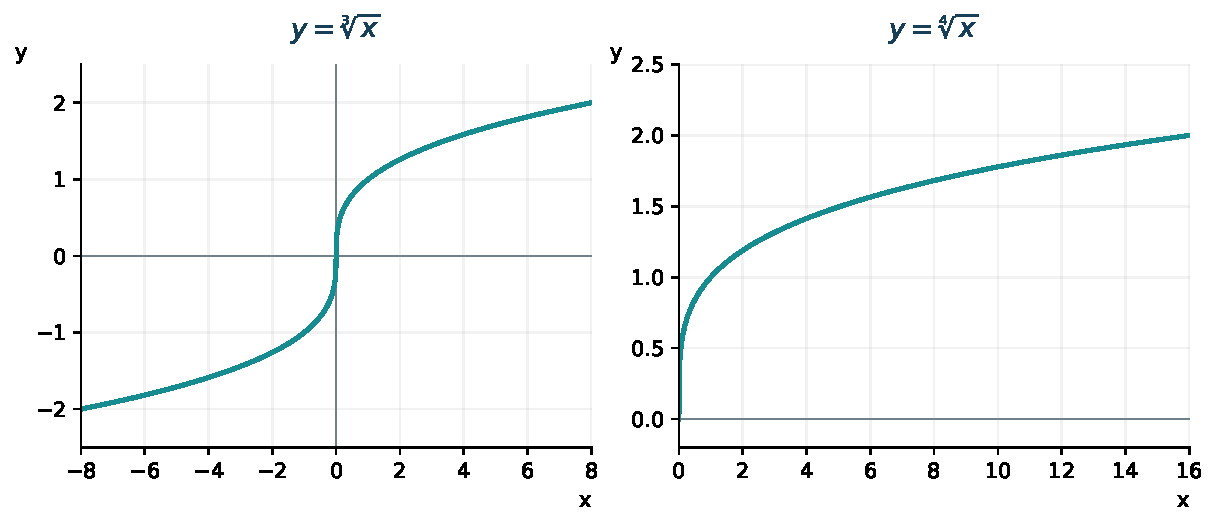
\includegraphics[width=\textwidth,height=.79\textheight,keepaspectratio]{images/atlas-roots.pdf}\par\small Корни нечётной и чётной степени\end{center}\end{minipage}\par
\Needspace{7\baselineskip}\section*{Задачи}
\begingroup\setlength{\parskip}{3pt}
\noindent\begin{minipage}[t]{\linewidth}\textbf{7.1.} Вычисли \(\sqrt{81}\) и \(\sqrt[3]{- 27}\).\par\end{minipage}\par
\noindent\begin{minipage}[t]{\linewidth}\textbf{7.2.} Вычисли \(\sqrt{\dfrac{49}{100}}\).\par\end{minipage}\par
\noindent\begin{minipage}[t]{\linewidth}\textbf{7.3.} Упрости \(\sqrt{72}\).\par\end{minipage}\par
\noindent\begin{minipage}[t]{\linewidth}\textbf{7.4.} Упрости \(\sqrt{200} - \sqrt{50}\).\par\end{minipage}\par
\par\addvspace{5pt}\begin{lrbox}{\CatFlowBox}\begin{minipage}[t]{\linewidth}
\setlength{\parskip}{5pt}\setlength{\columnsep}{4.5mm}\setlength{\intextsep}{0pt}
\begin{wrapfigure}[12]{r}{54mm}

\includegraphics[width=54mm,height=58mm,keepaspectratio]{images/unique/art-22.png}
\end{wrapfigure}
\textbf{7.5.} Внеси множитель под корень: \(3 \sqrt{5}\).\par

\textbf{7.6.} Вычисли \(\sqrt{12} \cdot  \sqrt{3}\).\par

\textbf{7.7.} Вычисли \(\dfrac{\sqrt{75}}{\sqrt{3}}\).\par

\textbf{7.8.} Вычисли \(\sqrt{(- 7)^{2}}\).\par

\textbf{7.9.} Между какими соседними целыми числами находится \(\sqrt{30}\)?\par

\textbf{7.10.} Сравни \(\sqrt{7}\) и \(2{,}7\).\par

\textbf{7.11.} Какие числа рациональные: \(\sqrt{16},\allowbreak \sqrt{2},\allowbreak - \dfrac{3}{7},\allowbreak 0{,}(3),\allowbreak \pi \)?\par
\par\WFclear\end{minipage}\end{lrbox}%
\ifdim\dimexpr\ht\CatFlowBox+\dp\CatFlowBox\relax<64mm\dp\CatFlowBox=\dimexpr64mm-\ht\CatFlowBox\relax\fi%
\noindent\usebox{\CatFlowBox}\par\addvspace{5pt}

\noindent\begin{minipage}[t]{\linewidth}\textbf{7.12.} Существуют ли \(\sqrt{- 9}\) и \(\sqrt[3]{- 8}\) в действительных числах?\par\end{minipage}\par
\noindent\begin{minipage}[t]{\linewidth}\textbf{7.13.} Квадратная комната имеет площадь \(49\) м\(^{2}\). Найди длину её стороны.\par\end{minipage}\par
\noindent\begin{minipage}[t]{\linewidth}\textbf{7.14.} Лестница стоит у стены: её основание в \(3\) м от стены, верх на высоте \(4\) м. Найди длину лестницы. Считай стену и землю перпендикулярными.\begin{center}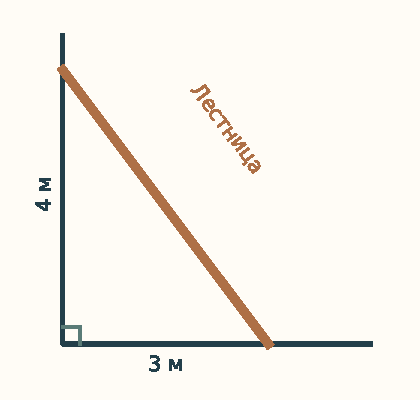
\includegraphics[width=.7\linewidth,height=45mm,keepaspectratio]{images/diagram-ladder.pdf}\end{center}\par\end{minipage}\par
\noindent\begin{minipage}[t]{\linewidth}\textbf{7.15.} У кубического контейнера объём \(0{,}125\) м\(^{3}\). Найди длину ребра в метрах и сантиметрах.\par\end{minipage}\par
\noindent\begin{minipage}[t]{\linewidth}\textbf{7.16.}\starmark{} Упрости: \(\sqrt{48} + \sqrt{75} - \sqrt{147}\).\par\end{minipage}\par
\noindent\begin{minipage}[t]{\linewidth}\textbf{7.17.}\starmark{} Проверь без десятичных приближений утверждение \(\sqrt{2} + \sqrt{3} > \sqrt{10}\). Докажи его или опровергни.\par\end{minipage}\par
\noindent\begin{minipage}[t]{\linewidth}\textbf{7.18.}\starmark{} У прямоугольника площадь \(48\) м\(^{2}\), одна сторона втрое длиннее другой. Найди обе стороны и диагональ.\par\end{minipage}\par
\noindent\begin{minipage}[t]{\linewidth}\textbf{7.19.} Докажите равенство \(\sqrt[n]{x^n}=|x|\) для любого действительного \(x\) и любого чётного натурального \(n\geq2\).\par\end{minipage}\par
\noindent\begin{minipage}[t]{\linewidth}\textbf{7.20.} Докажите, что для нечётного натурального \(n\geq3\) и любого действительного \(a\) выполнено \(\sqrt[n]{-a}=-\sqrt[n]a\).\par\end{minipage}\par
\noindent\begin{minipage}[t]{\linewidth}\textbf{7.21.} Вычислите \(\sqrt[4]{81}\), \(\sqrt[5]{-32}\) и \(\sqrt[6]{64}\).\par\end{minipage}\par
\par\addvspace{5pt}\begin{lrbox}{\CatFlowBox}\begin{minipage}[t]{\linewidth}
\setlength{\parskip}{5pt}\setlength{\columnsep}{4.5mm}\setlength{\intextsep}{0pt}
\begin{wrapfigure}[12]{l}{54mm}
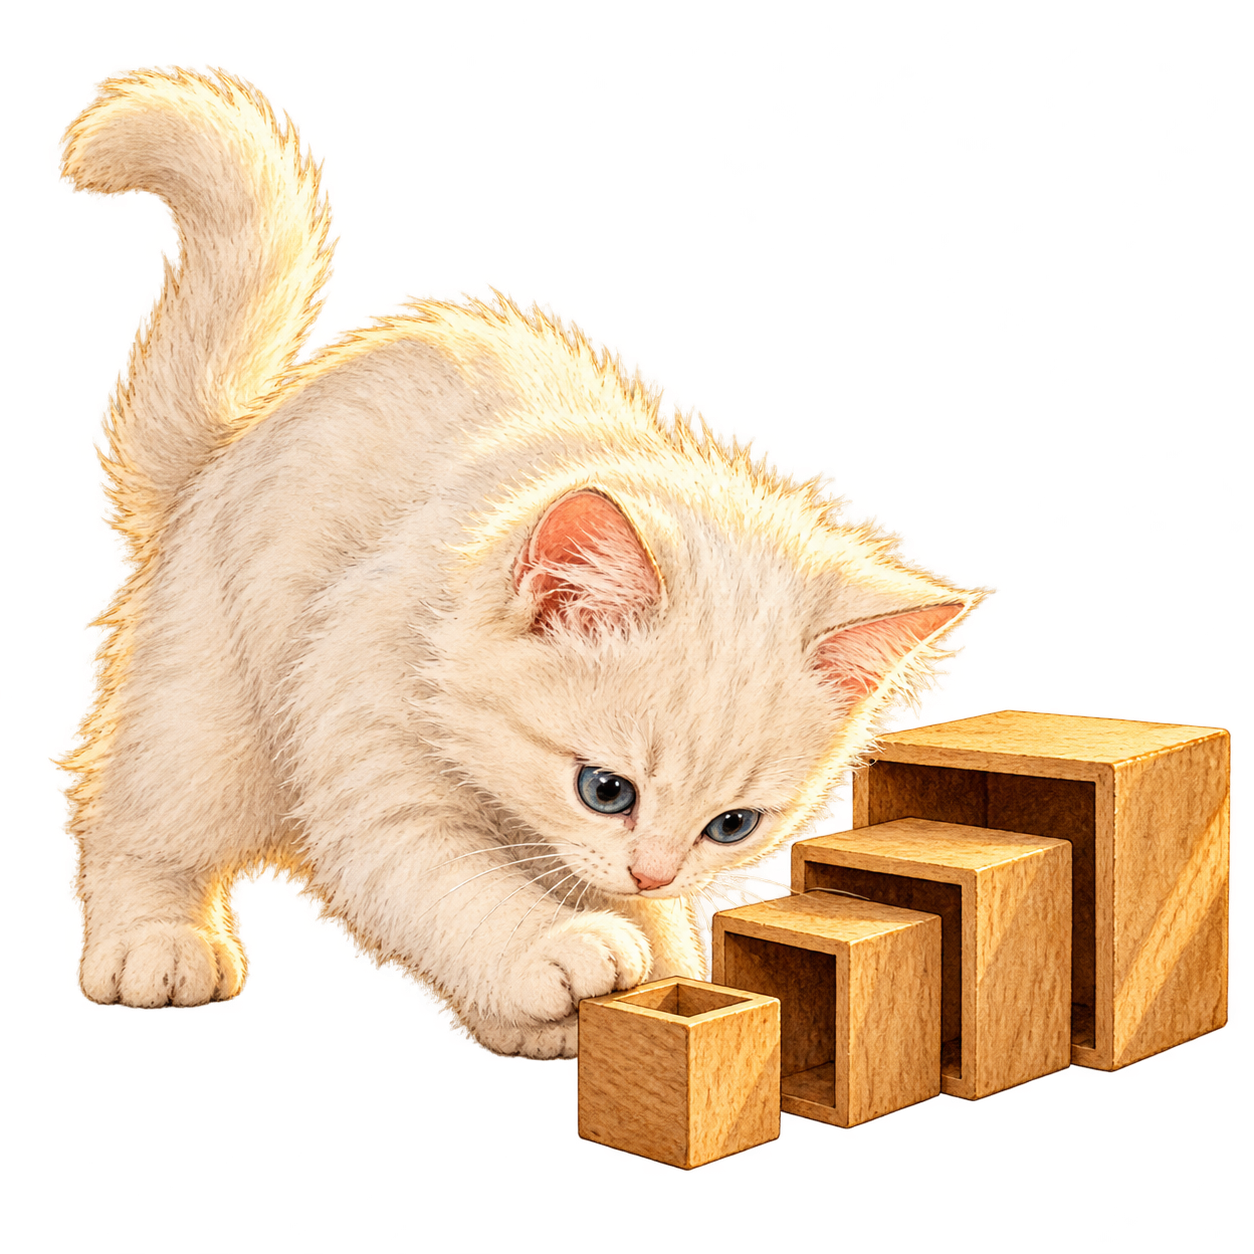
\includegraphics[width=54mm,height=58mm,keepaspectratio]{images/unique/art-15.png}
\end{wrapfigure}
\textbf{7.22.} Какие из выражений \(\sqrt[4]{-16}\), \(\sqrt[3]{-64}\), \(\sqrt[6]{0}\) определены в действительных числах? Вычислите определённые.\par

\textbf{7.23.} Упростите \(\sqrt[6]{x^6}\) и \(\sqrt[5]{x^5}\) для действительного \(x\).\par

\textbf{7.24.} Упростите \(\sqrt[4]{48}\) и вычислите \(\dfrac{\sqrt[3]{54}}{\sqrt[3]2}\).\par

\textbf{7.25.} Вычислите \((-32)^{\dfrac25}\), \((-8)^{-\dfrac13}\) и \(16^{-\dfrac34}\).\par

\textbf{7.26.} Решите в действительных числах \(\sqrt[4]{x+7}=2\) и \(\sqrt[3]{2x-1}=-3\).\par

\textbf{7.27.}\starmark{} Найдите область определения \(f(x)=\dfrac1{\sqrt[4]{x-2}}+\sqrt[3]{x+1}\).\par

\textbf{7.28.}\starmark{} Решите \(\sqrt[4]{(x-1)^4}=2-x\) в действительных числах.\par
\par\WFclear\end{minipage}\end{lrbox}%
\ifdim\dimexpr\ht\CatFlowBox+\dp\CatFlowBox\relax<64mm\dp\CatFlowBox=\dimexpr64mm-\ht\CatFlowBox\relax\fi%
\noindent\usebox{\CatFlowBox}\par\addvspace{5pt}

\endgroup
